% Copyright 2026 Sreeram Anil
% SPDX-License-Identifier: CC-BY-4.0
\chapter{Cost, memory and single-precision behaviour}
\label{ch:res-numerics}

\section{Execution time}

\Cref{tab:runtime} lists the measured cost per sample of every cell-level estimator on the
benchmark machine (one x86-64 core, GCC~13, \code{-O2}, SSE2 baseline, double precision;
minimum over repetitions as defined in \cref{sec:me-timing}), the ratio to the EKF, the size of
the estimator object, and the order-of-magnitude projection to a Cortex-M7 class flight
processor with the central factor $\kappa = 30$ of \cref{eq:me-scaling}.

% Copyright 2026 Sreeram Anil
% SPDX-License-Identifier: CC-BY-4.0
\begin{longtable}{llrrrr}
\caption{Computational cost per sample on the benchmark machine (x86-64, single core, g++ 13 -O2, double precision; median over runs) with the estimator object size, relative cost to the EKF, and an order-of-magnitude projection to a Cortex-M7 class flight processor using the central scaling factor $\kappa = 30$ of Chapter~\ref{ch:metrics} (range 20--90; a measurement on the target supersedes this column). Batch smoothers report the per-sample cost of the whole record.}\label{tab:runtime}\\
\toprule estimator & family & ns/step & $\times$EKF & bytes & est. Cortex-M7 [µs] \\ \midrule\endfirsthead
\toprule estimator & family & ns/step & $\times$EKF & bytes & est. Cortex-M7 [µs] \\ \midrule\endhead
CoulombCounting & baselines & 79 & 0.2 & 4184 & 2 \\
CoulombOCVHybrid & baselines & 211 & 0.4 & 4192 & 6 \\
OCVLookup & baselines & 1310 & 2.7 & 4192 & 39 \\
LKF & kalman & 334 & 0.7 & 4680 & 10 \\
EKF & kalman & 477 & 1.0 & 4336 & 14 \\
UD-EKF & kalman & 484 & 1.0 & 4480 & 15 \\
IEKF & kalman & 596 & 1.2 & 4336 & 18 \\
SR-EKF & kalman & 821 & 1.7 & 4440 & 25 \\
EIF & kalman & 1221 & 2.6 & 4472 & 37 \\
CKF & kalman & 1252 & 2.6 & 4560 & 38 \\
CDKF & kalman & 1375 & 2.9 & 4312 & 41 \\
UKF & kalman & 1442 & 3.0 & 4776 & 43 \\
SR-UKF & kalman & 1554 & 3.3 & 4896 & 47 \\
SCKF & kalman & 1581 & 3.3 & 4696 & 47 \\
IPLF & kalman & 2032 & 4.3 & 4784 & 61 \\
CKF5 & kalman & 4014 & 8.4 & 5624 & 120 \\
SO-EKF & kalman & 4202 & 8.8 & 4496 & 126 \\
GHKF & kalman & 11990 & 25.1 & 10784 & 360 \\
IAE-AKF & adaptive\_kalman & 500 & 1.0 & 5040 & 15 \\
Fading-EKF & adaptive\_kalman & 501 & 1.0 & 4384 & 15 \\
STF & adaptive\_kalman & 532 & 1.1 & 4680 & 16 \\
SageHusa-AKF & adaptive\_kalman & 545 & 1.1 & 4808 & 16 \\
Fuzzy-AKF & adaptive\_kalman & 727 & 1.5 & 4816 & 22 \\
VB-AKF & adaptive\_kalman & 872 & 1.8 & 4408 & 26 \\
MMAE & adaptive\_kalman & 1752 & 3.7 & 13200 & 53 \\
IMM & adaptive\_kalman & 2076 & 4.4 & 4976 & 62 \\
ReducedOrder-EKF & robust\_kalman & 331 & 0.7 & 4272 & 10 \\
SVSF & robust\_kalman & 583 & 1.2 & 4376 & 17 \\
Constrained-EKF & robust\_kalman & 586 & 1.2 & 4416 & 18 \\
Huber-EKF & robust\_kalman & 642 & 1.3 & 4368 & 19 \\
StudentT-KF & robust\_kalman & 696 & 1.5 & 4568 & 21 \\
Hinf-EKF & robust\_kalman & 798 & 1.7 & 4408 & 24 \\
MC-EKF & robust\_kalman & 998 & 2.1 & 4384 & 30 \\
Schmidt-KF & robust\_kalman & 1293 & 2.7 & 8856 & 39 \\
SuperTwisting-SMO & observers & 142 & 0.3 & 4280 & 4 \\
SSKF & observers & 416 & 0.9 & 4632 & 12 \\
Luenberger & observers & 478 & 1.0 & 4632 & 14 \\
HGO & observers & 479 & 1.0 & 4680 & 14 \\
SMO-Adaptive & observers & 511 & 1.1 & 4800 & 15 \\
SMO & observers & 517 & 1.1 & 4800 & 16 \\
UIO & observers & 581 & 1.2 & 5072 & 17 \\
DOB & observers & 587 & 1.2 & 4784 & 18 \\
IntervalObserver & observers & 808 & 1.7 & 9024 & 24 \\
AdaptiveObserver & observers & 900 & 1.9 & 4864 & 27 \\
PI-Observer & observers & 1373 & 2.9 & 4824 & 41 \\
ESO & observers & 1479 & 3.1 & 4784 & 44 \\
AWTLS & soh & 483 & 1.0 & 8776 & 14 \\
RLS-EKF & soh & 496 & 1.0 & 8904 & 15 \\
JointEKF & soh & 1215 & 2.5 & 8752 & 36 \\
DualEKF & soh & 1272 & 2.7 & 4752 & 38 \\
DualUKF & soh & 2371 & 5.0 & 5512 & 71 \\
JointUKF & soh & 3103 & 6.5 & 9600 & 93 \\
GSF & particle & 1749 & 3.7 & 9192 & 52 \\
EnKF & particle & 10283 & 21.6 & 6776 & 308 \\
ETKF & particle & 10551 & 22.1 & 5304 & 317 \\
PF-Fast & particle & 15960 & 33.5 & 9664 & 479 \\
UPF & particle & 18614 & 39.0 & 25360 & 558 \\
RBPF & particle & 39896 & 83.7 & 34016 & 1197 \\
PF-Bootstrap & particle & 76444 & 160.3 & 46472 & 2293 \\
PF-Regularized & particle & 81850 & 171.7 & 46464 & 2456 \\
PF-Auxiliary & particle & 104352 & 218.8 & 54584 & 3131 \\
NN-Direct & learning & 484 & 1.0 & 15152 & 15 \\
NN-EKF & learning & 1059 & 2.2 & 4376 & 32 \\
ELM-RLS-EKF & learning & 3292 & 6.9 & 11704 & 99 \\
MHE-RTI & optimization & 17270 & 36.2 & 26928 & 518 \\
MHE & optimization & 32403 & 68.0 & 26928 & 972 \\
ERTS & smoothers & 907 & 1.9 & 12.5\,MB & 27 \\
URTS & smoothers & 2473 & 5.2 & 12.5\,MB & 74 \\
Batch-NLS & smoothers & 4662 & 9.8 & 17.4\,MB & 140 \\
FixedLag-EKF & smoothers & 9915 & 20.8 & 19992 & 297 \\
\bottomrule\end{longtable}


The table spans three orders of magnitude and falls into four bands. Below
\SI{1}{\micro\second} per step are Coulomb counting (\SI{79}{\nano\second}), the
super-twisting observer (\SI{141}{\nano\second}), the reduced-order EKF, the linear KF, the
Luenberger-type observers, the EKF (\SI{477}{\nano\second}) and its adaptive and robust
variants, the dual EKF-class SOH estimators, the direct neural regressor and the U-D filter.
Between \SI{1}{} and \SI{5}{\micro\second} are the sigma-point and cubature filters
(\SIrange{1.25}{1.6}{\micro\second}, three times the EKF, for the $2n_x+1 = 9$ or $2n_x = 8$
model evaluations per step), the information and square-root forms, the IMM, MMAE, the
Schmidt filter, the joint filters, the Gaussian-sum filter, ELM-RLS-EKF and the second-order
and fifth-degree filters. Between \SI{10}{} and \SI{40}{\micro\second} are the Gauss--Hermite
filter ($3^4 = 81$ points, \SI{12}{\micro\second}), the ensemble filters, PF-Fast, the UPF, the
two MHE variants (\SI{17}{} and \SI{32}{\micro\second}) and the RBPF. Above
\SI{75}{\micro\second} are the three 500-particle bootstrap-type filters, of which the
auxiliary PF at \SI{104}{\micro\second} is the most expensive estimator in the library, 219
times the EKF.

On a \SI{10}{\hertz} BMS schedule the projection to a flight processor puts every estimator of
the first two bands below \SI{0.2}{\percent} of one core per cell (the EKF at
\SI{0.014}{\percent}), the twelve-cell decentralised EKF of \cref{ch:res-pack} at about
\SI{0.2}{\percent}, MHE at \SI{1}{\percent}; the 500-particle filters reach
\SIrange{2}{3}{\percent} per cell and are the only family for which the arithmetic budget of a
module-level controller is a real constraint. The batch smoothers (\SIrange{0.9}{4.7}{\micro\second}
per sample when amortised over the record, but \SIrange{12}{17}{\mega\byte} of storage) and the
fixed-lag smoother (\SI{9.9}{\micro\second}, \SI{20}{\kilo\byte}) are post-flight tools by
construction.

\Cref{fig:res-runtime} in \cref{ch:res-cell_ecm} already made the point that matters: below
\SI{2}{\micro\second} per step the cost axis does not discriminate the estimators, because the
best twelve of the composite ranking all lie in that range. Cost becomes an argument only
between families --- a particle filter against a sigma-point filter, MHE against an adaptive
EKF --- and in those comparisons the cheaper estimator is, on this problem, at least as
accurate.

\section{Memory}

The \code{bytes} column of \cref{tab:runtime} is \code{sizeof} of the complete estimator
object. For every filter over the equivalent-circuit model it is dominated by the model copy
that each templated filter carries, and in the model by the 241-point OCV table with its slopes
(\SI{3.9}{\kilo\byte} of the \SI{4.3}{\kilo\byte} of an EKF, \cref{tab:me-mem}); the filter
state proper is \SI{200}{\byte} for the EKF, \SI{700}{\byte} for the UKF, \SI{5}{\kilo\byte} for
the Schmidt filter with its consider-state cross-covariance, \SI{22}{\kilo\byte} for MHE (a
window of 21 states with their Jacobians) and \SIrange{42}{50}{\kilo\byte} for the 500-particle
filters. A production build shares one OCV table across all cells of a module, which reduces
the per-cell footprint of the Kalman-type estimators to under a kilobyte and makes the
twelve-cell decentralised EKF a \SI{6}{\kilo\byte} object rather than the \SI{52}{\kilo\byte}
reported. No estimator in the library allocates memory after construction; the numbers in the
table are the static budget.

\section{Single precision}

\Cref{tab:float} repeats the equivalent-circuit benchmark (seed~1, eVTOL mission, all twelve
scenarios) with the library compiled for \code{float}, and lists four scenarios next to their
double-precision counterparts; \cref{fig:res-float} plots the ratio of the two for every
estimator. The question the experiment answers is whether any estimator \emph{needs} double
precision on this problem.

% Copyright 2026 Sreeram Anil
% SPDX-License-Identifier: CC-BY-4.0
\begin{longtable}{lrrrrrrrr}
\caption{Single-precision (float32) build versus double precision: steady-state SOC RMSE [\%] (seed 1, ECM plant, eVTOL). A large ratio indicates loss of numerical robustness in float32; `div' marks divergence.}\label{tab:float}\\
\toprule estimator & \multicolumn{2}{c}{nominal} & \multicolumn{2}{c}{init\_error} & \multicolumn{2}{c}{aged\_cell} & \multicolumn{2}{c}{combined} \\
 & f64 & f32 & f64 & f32 & f64 & f32 & f64 & f32 \\ \midrule\endfirsthead
\toprule estimator & \multicolumn{2}{c}{nominal} & \multicolumn{2}{c}{init\_error} & \multicolumn{2}{c}{aged\_cell} & \multicolumn{2}{c}{combined} \\ \midrule\endhead
CoulombCounting & 0.36 & 0.36 & 35.35 & 35.35$^{\mathrm{div}}$ & 10.06 & 10.06 & 20.93 & 20.93 \\
OCVLookup & 1.31 & 1.31 & 1.31 & 1.31 & 1.37 & 1.37 & 1.14 & 1.14 \\
CoulombOCVHybrid & 0.17 & 0.17 & 4.43 & 4.43 & 9.44 & 9.44 & 1.33 & 1.33 \\
EKF & 0.06 & 0.06 & 0.05 & 0.04 & 1.39 & 1.48 & 11.90 & 12.21 \\
UKF & 0.04 & 0.05 & 0.06 & 0.04 & 1.50 & 0.92 & 1.79 & 1.07 \\
LKF & 1.19 & 1.19 & 2.20 & 2.17 & 1.15 & 1.15 & 7.04 & 7.04 \\
IEKF & 0.13 & 0.03 & 0.07 & 0.03 & 1.47 & 1.79 & 2.48 & 1.83 \\
CKF & 0.05 & 0.05 & 0.09 & 0.09 & 2.51 & 2.53 & 12.94 & 12.97 \\
SCKF & 0.05 & 0.05 & 0.09 & 0.09 & 2.51 & 2.48 & 12.94 & 12.84 \\
CKF5 & 0.05 & 0.05 & 0.11 & 0.11 & 1.84 & 2.39 & 14.57 & 14.59 \\
CDKF & 0.05 & 0.04 & 0.11 & 0.10 & 1.84 & 2.24 & 14.57 & 14.59 \\
GHKF & 0.05 & 0.02 & 0.11 & 0.06 & 1.84 & 1.96 & 14.57 & 14.56 \\
IPLF & 0.07 & 0.06 & 0.03 & 0.04 & 2.28 & 1.61 & 1.79 & 1.86 \\
EIF & 0.06 & 0.03 & 0.05 & 0.06 & 1.39 & 1.40 & 11.90 & 12.66 \\
SR-EKF & 0.06 & 0.06 & 0.05 & 0.05 & 1.39 & 1.47 & 11.90 & 12.21 \\
SR-UKF & 0.04 & 0.14 & 0.06 & 0.04 & 1.50 & 0.96 & 1.79 & 0.23 \\
UD-EKF & 0.06 & 0.06 & 0.05 & 0.04 & 1.39 & 1.48 & 11.90 & 12.18 \\
SO-EKF & 0.03 & 0.07 & 0.08 & 0.06 & 1.79 & 1.45 & 1.12 & 1.36 \\
SageHusa-AKF & 0.05 & 0.06 & 0.06 & 0.05 & 1.14 & 1.12 & 1.95 & 1.95 \\
IAE-AKF & 0.03 & 0.05 & 0.06 & 0.09 & 1.23 & 1.15 & 2.01 & 2.02 \\
VB-AKF & 0.05 & 0.03 & 0.03 & 0.04 & 1.19 & 1.19 & 2.00 & 1.95 \\
STF & 0.09 & 0.09 & 0.09 & 0.09 & 2.74 & 2.75 & 2.71 & 2.72 \\
Fading-EKF & 0.06 & 0.06 & 0.06 & 0.06 & 1.78 & 1.78 & 1.17 & 1.17 \\
Fuzzy-AKF & 0.04 & 0.06 & 0.02 & 0.06 & 1.20 & 1.28 & 2.29 & 2.29 \\
IMM & 0.06 & 0.06 & 0.03 & 0.08 & 0.84 & 0.83 & 0.89 & 0.57 \\
MMAE & 0.33 & 0.37 & 0.37 & 0.35 & 1.99 & 2.29 & 12.03 & 12.30 \\
Schmidt-KF & 0.51 & 0.51 & 0.51 & 0.51 & 0.56 & 0.56 & 1.17 & 1.16 \\
Hinf-EKF & 0.03 & 0.02 & 0.02 & 0.02 & 0.92 & 0.88 & 4.81 & 7.26 \\
Huber-EKF & 0.06 & 0.05 & 0.03 & 0.08 & 1.84 & 1.71 & 4.43 & 4.18 \\
MC-EKF & 0.08 & 0.03 & 0.03 & 0.05 & 1.44 & 1.20 & 3.31 & 3.65 \\
StudentT-KF & 0.04 & 0.04 & 0.04 & 0.03 & 1.57 & 1.59 & 4.26 & 3.53 \\
Constrained-EKF & 0.06 & 0.06 & 0.05 & 0.05 & 1.40 & 1.44 & 12.87 & 12.85 \\
ReducedOrder-EKF & 0.08 & 0.08 & 0.08 & 0.08 & 2.11 & 2.11 & 1.68 & 1.68 \\
SVSF & 0.04 & 0.05 & 0.04 & 0.03 & 1.06 & 1.03 & 1.99 & 1.98 \\
Luenberger & 0.08 & 0.08 & 0.08 & 0.08 & 2.17 & 2.17 & 2.15 & 2.15 \\
SSKF & 0.08 & 0.08 & 0.08 & 0.08 & 2.17 & 2.17 & 2.03 & 2.03 \\
PI-Observer & 0.09 & 0.10 & 0.09 & 0.10 & 2.69 & 2.79 & 1.81 & 2.16 \\
SMO & 0.08 & 0.08 & 0.08 & 0.08 & 2.21 & 2.21 & 2.07 & 2.07 \\
SMO-Adaptive & 0.08 & 0.08 & 0.08 & 0.08 & 2.19 & 2.19 & 2.09 & 1.95 \\
SuperTwisting-SMO & 0.09 & 0.09 & 0.09 & 0.09 & 2.48 & 2.48 & 2.44 & 2.44 \\
HGO & 0.08 & 0.08 & 0.08 & 0.08 & 2.17 & 2.18 & 2.16 & 2.01 \\
ESO & 0.10 & 0.10 & 0.10 & 0.10 & 2.64 & 2.64 & 2.79 & 2.23 \\
UIO & 0.07 & 0.07 & 0.07 & 0.07 & 1.89 & 1.91 & 1.78 & 1.85 \\
DOB & 0.02 & 0.02 & 0.24 & 0.24 & 1.97 & 1.97 & 2.35 & 2.30 \\
AdaptiveObserver & 0.05 & 0.05 & 0.05 & 0.05 & 1.10 & 1.10 & 0.78 & 0.81 \\
IntervalObserver & 0.08 & 0.08 & 0.08 & 0.08 & 2.17 & 2.17 & 2.03 & 2.03 \\
JointEKF & 0.05 & 0.08 & 0.05 & 0.08 & 0.02 & 0.02 & 2.37 & 2.55 \\
JointUKF & 0.11 & 0.06 & 0.09 & 0.08 & 0.07 & 0.08 & 1.91 & 2.13 \\
DualEKF & 0.02 & 0.12 & 0.08 & 0.10 & 0.62 & 0.60 & 2.21 & 1.86 \\
DualUKF & 0.06 & 0.05 & 0.05 & 0.16 & 0.14 & 0.09 & 2.02 & 1.96 \\
RLS-EKF & 0.54 & 0.51 & 0.49 & 0.46 & 4.25 & 4.29 & 3.01 & 3.28 \\
AWTLS & 0.01 & 0.02 & 0.01 & 0.01 & 0.51 & 0.55 & 8.93 & 9.25 \\
PF-Bootstrap & 0.18 & 0.17 & 0.09 & 0.13 & 2.52 & 2.50 & 2.92 & 2.52 \\
PF-Fast & 0.22 & 0.22 & 0.16 & 0.19 & 2.59 & 2.60 & 2.37 & 3.01 \\
PF-Regularized & 0.09 & 0.08 & 0.11 & 0.12 & 2.40 & 2.50 & 2.66 & 2.73 \\
PF-Auxiliary & 0.13 & 0.13 & 0.14 & 0.17 & 2.40 & 2.46 & 1.92 & 2.19 \\
RBPF & 0.06 & 0.05 & 0.37 & 0.39 & 2.21 & 2.12 & 2.03 & 1.67 \\
UPF & 0.42 & 0.48 & 0.41 & 0.45 & 2.80 & 2.66 & 2.33 & 2.77 \\
EnKF & 0.25 & 0.25 & 0.25 & 0.25 & 1.91 & 1.96 & 6.97 & 6.97 \\
ETKF & 0.26 & 0.25 & 0.88 & 0.89 & 3.51 & 3.52 & 2.57 & 2.53 \\
GSF & 0.06 & 0.03 & 0.11 & 0.06 & 3.35 & 3.03 & 3.63 & 3.15 \\
NN-Direct & 1.17 & 1.17 & 1.17 & 1.17 & 1.78 & 1.79 & 4.10 & 4.10 \\
NN-EKF & 0.28 & 0.28 & 0.28 & 0.28 & 1.41 & 1.43 & 11.16 & 11.99 \\
ELM-RLS-EKF & 0.02 & 0.05 & 0.02 & 0.02 & 1.37 & 1.74 & 11.69 & 12.54 \\
MHE-RTI & 0.08 & 0.08 & 0.13 & 0.11 & 0.81 & 0.79 & 0.55 & 0.50 \\
MHE & 0.10 & 0.10 & 0.10 & 0.08 & 0.81 & 0.81 & 0.68 & 0.59 \\
ERTS & 0.04 & 0.04 & 0.04 & 0.04 & 1.59 & 1.55 & 10.72 & 12.04 \\
URTS & 0.04 & 0.07 & 0.04 & 0.01 & 1.54 & 1.94 & 0.70 & 0.50 \\
Batch-NLS & 0.04 & 0.04 & 0.04 & 0.04 & 2.00 & 1.63 & 3.74 & 4.52 \\
FixedLag-EKF & 0.04 & 0.04 & 0.04 & 0.04 & 1.42 & 1.51 & 11.87 & 12.22 \\
\bottomrule\end{longtable}


\begin{figure}[H]\centering
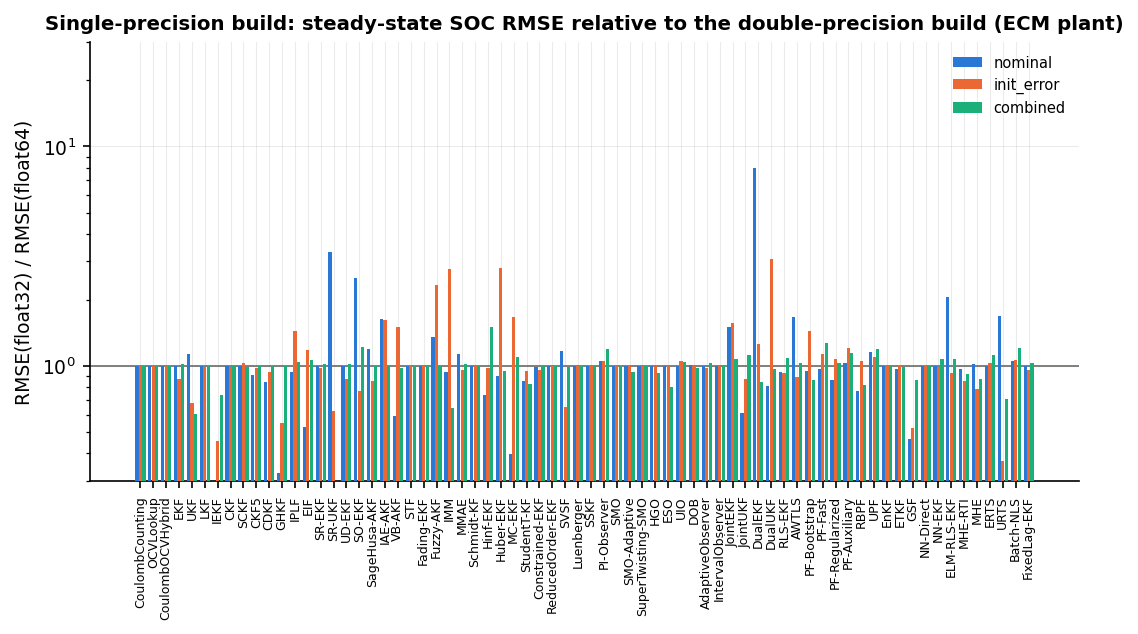
\includegraphics[width=\textwidth]{figures/overview_float_vs_double.png}
\caption{Ratio of the steady-state RMSE of the single-precision build to the double-precision
build, ECM plant, seed~1. A ratio of one is identical behaviour; ratios below one are as
common as ratios above it.}
\label{fig:res-float}
\end{figure}

The answer is that none does. Over the 840 float32 runs no estimator diverges that did not
also diverge in double precision (Coulomb counting on \code{init\_error}, which has nothing to
do with arithmetic). In 406 of the 840 runs the steady-state RMSE agrees with the double build
to within \num{0.005} percentage points, the median absolute difference over all runs is
\num{0.006} points, and the differences above \num{0.25} points are confined to the scenarios in
which the seed-to-seed spread of the double build is itself large --- \code{combined},
\code{aged\_cell}, \code{param\_mismatch}, \code{cold} and \code{outliers} --- and are of both
signs: the SR-UKF improves from \num{1.79} to \num{0.23} on \code{combined} in float, the
$H_\infty$ filter degrades from \num{4.81} to \num{7.26}, the joint EKF improves from \num{2.09}
to \num{0.80} on \code{param\_mismatch}, the ERTS degrades from \num{10.72} to \num{12.04} on
\code{combined}. These are not precision losses in the Verhaegen--Van~Dooren sense
(\cref{sec:me-float}); they are the sensitivity of a run that is already on the edge of
failure to any perturbation, of which rounding is one. The single-precision build also
regenerates the data set in single precision, so its noise realisation is not bit-identical to
the double build's, and on \code{outliers} in particular a different outlier draw moves the
EKF-type filters by \num{0.3} points --- within the range that the three double-precision seeds
span.

The Verhaegen--Van~Dooren argument predicted that the conventional covariance form would lose
accuracy before the factorised forms at the $\kappa(\mP) \sim 10^6$ condition numbers the cell
model produces. The benchmark does not confirm it for this model: the EKF, its square-root form
and its U-D form are within \num{0.03} points of each other in float in every column of
\cref{tab:float}, and the UKF and SR-UKF within \num{0.1} points except on \code{combined},
where the SR-UKF is better by luck rather than by arithmetic. The reason is that the covariance of the cell filter
is small in absolute terms ($\mP_{\soc\soc} \sim 10^{-6}$ after convergence) and the library's
EKF uses the Joseph-form update by default and every filter re-symmetrises its covariance
after each step, which keeps the conventional recursion positive definite in binary32 at these
condition numbers. The factorised forms remain
the right choice where the state dimension or the dynamic range of the covariance grows --- the
pack-level joint filters, an attitude filter with a bias state --- and their cost premium
(\SI{72}{\percent} for the SR-EKF, \SI{8}{\percent} for the SR-UKF, \SI{2}{\percent} for the U-D
filter) is the price of not having to find out.

The one systematic effect of single precision is speed. On the benchmark machine the float
build runs the median estimator in \SI{77}{\percent} of the double build's time (the EKF in
\SI{75}{\percent}, the UKF in \SI{73}{\percent}, MHE in \SI{66}{\percent}, the fixed-lag smoother
in \SI{35}{\percent}); on a Cortex-M4F or a single-precision-only M7 the ratio is an order of
magnitude, because \code{double} is emulated in software. The practical conclusion for a
flight implementation is the one \cref{sec:me-float} anticipated: build the library for
\code{float}, keep the Joseph-form update and the symmetrisation, and reserve the square-root
forms for estimators whose covariance dynamic range justifies them.

\section{Determinism and unit tests}

The library has no data-dependent branches that allocate, no recursion and no exceptions. The
unit-test executable (\code{tests/unit\_tests.cpp}) exercises the linear algebra (Cholesky
factorisation and rank-one updates, the Ackermann and conditioned pole-placement routines,
both DARE solvers against the Riccati residual), the analytic model Jacobians against central
differences (double build only, since the finite-difference truncation error exceeds the
tolerance in binary32), the plants (OCV monotonicity and end points, the thermal balance, the
single-particle model against the OCV at rest, the orientation of the Preisach loop) and the
convergence of the EKF and UKF on the \code{init\_error} mission; it passes in both
precisions (\cref{app:build}). Every benchmark run is reproducible bit for bit from its seed,
which is what allowed the per-estimator chapters to quote single-seed traces and the tables to
be regenerated from the recorded summaries.
